\documentclass[a4paper,12pt,abstracton]{scrartcl}
\usepackage[ngerman, english]{babel}
\usepackage[utf8]{inputenc}
\usepackage[T1]{fontenc}
\usepackage{graphicx}
\usepackage{lipsum}
\usepackage{blindtext}

\title{Bachelorarbeit}
\author{Sophia Milanov}
\date{\today}

\begin{document}

\begin{titlepage}
\begin{center}
 
\Large\textbf{Department of Physics and Astronomy\\
University of Heidelberg}

\vspace{16cm}

\normalsize
Bachelor Thesis in Physics\\
submitted by \\
\vspace{0.5cm}
\Large\textbf{Sophia Milanov}\\
\normalsize
\vspace{0.5cm}
born in Düsseldorf (Germany)\\
\vspace{0.5cm}
\Large\textbf{2016}
\normalsize

\newpage




\Large\textbf{Title}

\vspace{18cm}

\normalsize
This Bachelor Thesis has been carried out by Sophia Milanov at the\\
Max Planck Institute for Astronomy in Heidelberg\\
under the supervision of\\
Dr. Glenn van de Ven

\vfill
\end{center}

\end{titlepage}


\begin{abstract}
\Blindtext 
\end{abstract}

\newpage

\tableofcontents

\newpage
\part{Introduction}
\section{What is a globular cluster in the Milky Way?}
150 of them \\
kugelförmige anordnung von Sternen 10**6 bis 10**8\\
große frage: IMBHs ja/nein
\section{Poisson's equation}
\section{Models of globular clusters}
\subsection{CMD}
color magnitude diagram aussage\\
alter\\
metallicity\\
star formation\\
\begin{figure}[htbp] 
	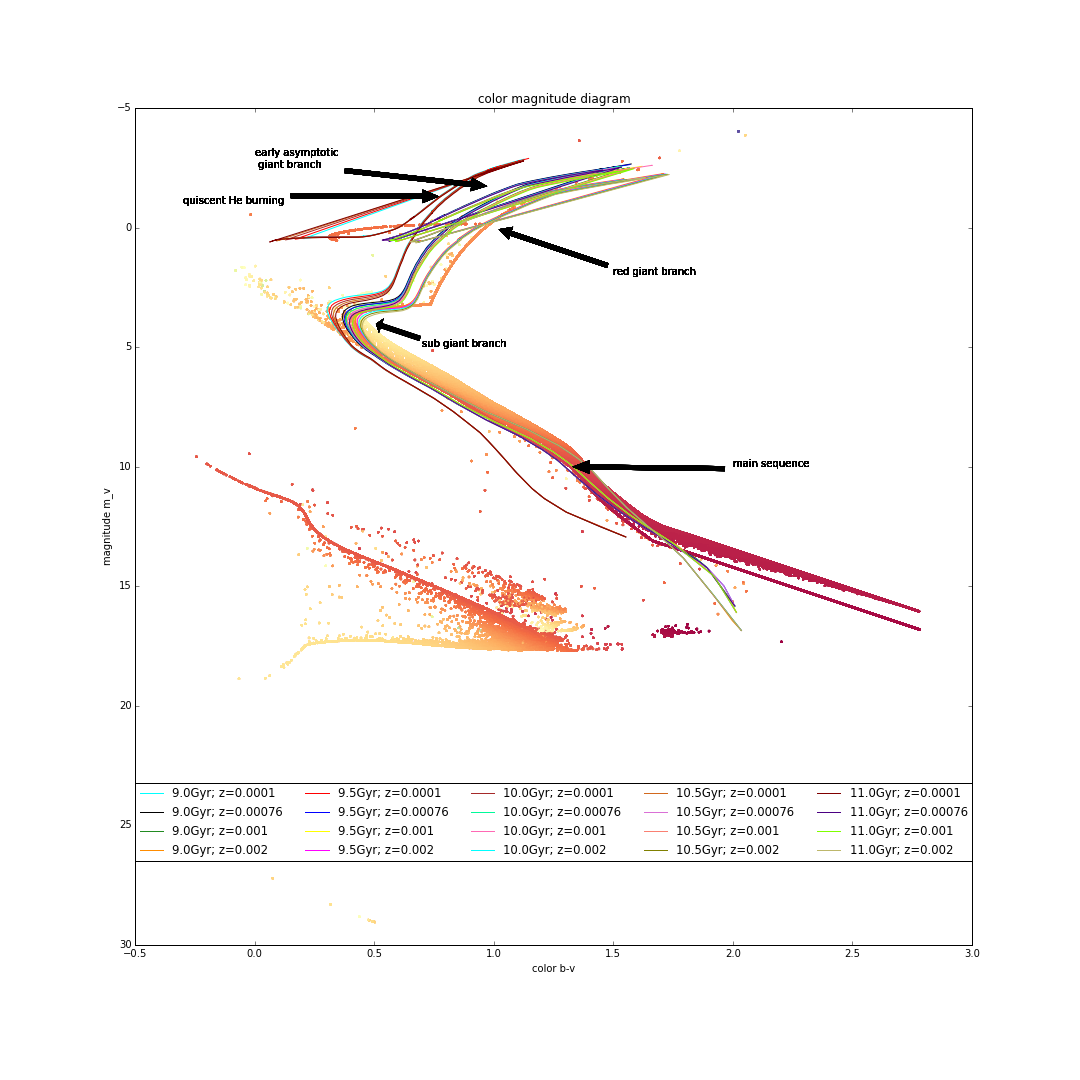
\includegraphics[width=\textwidth]{./Plots/color_magnitude_diagram_with_iscochrones.png}
	\caption{cmd isochrones}
	\label{fig:Abbildung1} 
\end{figure}
\subsection{Velocity dispersion}
aussage\\
plots\\
erklärung physikalisch
\subsection{Density profile}
plots\\
bestätigung kugelförmig\\
potential daraus
\subsection{Potential}
\section{Orbits}

\newpage
\part{Analysis}
\newpage
\part{Discussion}
\end{document}